% main.tex -- Paper B (design study, simulation only). REVTeX 4.2, APS style.
% ALL device numbers are SIMULATION results. Sources (relative to ../):
%   data/results_B.json (operating point, source powers, spectrum, thermal), data/eff_vs_power.csv (Fig. 1a),
%   data/Q_tolerance.csv, data/RF_detuning.csv, data/IDT_sensitivity.csv (Fig. 2),
%   data/HOM.csv (AUTHORITATIVE delay-matched HOM; identical to the regenerated "HOM" block of results_B.json, checked 2026-10-07 20:50)
% Scripts: core.py, make_all.py, hom_post.py. Literature numbers: see per-entry verification comments in refs.bib.
\documentclass[aps,prapplied,reprint,superscriptaddress,amsmath,amssymb,floatfix]{revtex4-2}
\usepackage{graphicx}
\usepackage{bm}
\usepackage[colorlinks=true,linkcolor=blue,citecolor=blue,urlcolor=blue]{hyperref}
\newcommand{\etash}{\eta_{\rm shift}}
\newcommand{\etaabs}{\eta_{\rm abs}}
\newcommand{\Pg}{P_{\rm RF}}

\begin{document}

\title{Acoustically driven coupled-ring single-photon frequency shifter on thin-film lithium niobate: a design study}

\author{Xinlei Chen}
\author{Yuanhua Li}
% TODO: confirm college/department, postcode, corresponding author and e-mail.
\affiliation{Shanghai University of Electric Power, Shanghai, China}

\date{\today}

\begin{abstract}
We present a simulation-only design study of a single-photon frequency shifter on thin-film lithium niobate (TFLN) in which a suspended interdigital-transducer (IDT) acoustic resonator, instead of electrodes, drives one ring of a coupled-ring photonic molecule. Integrating the full time-domain coupled-mode equations without the rotating-wave approximation, with the drive calibrated to a measured resonant acousto-optic modulator and the measured intrinsic quality factor $Q_i\approx2.4\times10^6$ of that platform, we find that the device sends 98.3\% of the output light into a single sideband 3.33~GHz away, using $\approx$7~$\mu$W (6.7~$\mu$W) of source RF power, with 55\% absolute efficiency and 2.5~dB insertion loss. The best published acousto-optic frequency shifter on TFLN reaches 3.5\% on-chip efficiency at 1~W (30~dBm). The design does \emph{not}, however, offer a power advantage over electro-optic (EO) driving: once both drives are impedance matched, their source powers differ by only a factor of 0.36--3.9, and an LC-matched EO drive with a low-loss inductor needs \emph{less} power. The acoustic drive also loses to an LC-matched EO drive if the IDT efficiency falls below $\approx$25\%, and its usable RF bandwidth is only $\sim$1~MHz. For a quantum interface we compute the Hong--Ou--Mandel (HOM) visibility with a delay-matched reference photon: after filtering the target frequency bin, $1-V=8\times10^{-7}$ ($V=0.9999992$) for a 10-MHz-bandwidth photon and $6\times10^{-4}$ at 50~MHz, whereas without filtering the residual carrier and spurious orders limit the visibility to $V=0.9835$, so a target-bin filter is required. Because the process is pump-free and number-conserving, thermal phonons contribute a negligible incoherent coupling noise ($n_{\rm th}/N_{\rm coh}\approx10^{-8}$) even at room temperature.
\end{abstract}

\maketitle

\begin{figure*}[t]
\centering
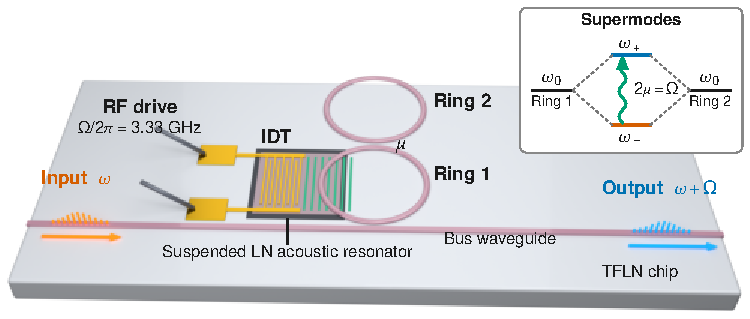
\includegraphics[width=5.0in]{figures/fig1_device.pdf}
\caption{Device concept. An RF-driven interdigital transducer (IDT; $\Omega/2\pi=3.33$~GHz) excites a suspended LN acoustic resonator that covers only a segment of ring~1. Ring~2 is coupled only to ring~1 (coupling rate $\mu$), and a single bus waveguide is coupled only to ring~1. Light enters in the forward direction at $\omega$ and leaves the same bus at the shifted frequency $\omega+\Omega$. Inset: the ring--ring coupling splits the two degenerate ring modes ($\omega_0$) into supermodes $\omega_\pm$ separated by $2\mu=\Omega$, which the acoustic drive couples. Schematic, not to scale.}
\label{fig:device}
\end{figure*}


% ================================================================ Introduction
\section{Introduction}
Photonic qubits encoded in discrete frequency bins need low-loss, coherent devices that move single photons between bins~\cite{Lukens2017,Kues2017,Lu2018}. TFLN combines strong Pockels, piezoelectric, and photoelastic responses with low-loss resonators~\cite{Wang2018,Zhang2017}, and has been used for single-photon spectral shearing over $\pm641$~GHz~\cite{Zhu2022}, an integrated quantum frequency processor~\cite{Yang2026}, and coupled-cavity frequency beam splitters~\cite{Cohen2026}. For single-tone shifting, the benchmark is the EO coupled-ring shifter of Hu \emph{et al.}~\cite{Hu2021}: a microwave drive couples the symmetric (S) and antisymmetric (AS) supermodes of a photonic molecule~\cite{Zhang2019} and, at a generalized critical-coupling condition, transfers light unidirectionally from one supermode to the other. The measured device shifts 98.7\% of the output light by 28.2~GHz with 0.45~dB insertion loss (IL), and 99.1\% (up) and 99.4\% (down) at 12.5~GHz, using 96~mW of microwave power~\cite{Hu2021}. A different EO approach, serrodyne driving of cascaded traveling-wave TFLN phase modulators, reports a shifting efficiency above 98.8\% with $V_\pi\approx2.3$~V~\cite{Qiu2025}.% Qiu2025: values from published abstract (Optica landing page, Crossref, Engineering Village record).

Acoustic frequency shifting on TFLN is much less mature. The best published TFLN acousto-optic frequency shifter, a traveling-wave Bragg-deflection device at $\sim$3~GHz, reaches an on-chip efficiency of 3.5\% at 30~dBm (1~W) applied to the IDT pads, with $>$30~dB carrier suppression and a 70-MHz microwave bandwidth~\cite{Shao2020}. Resonant acoustics improves the per-volt modulation strongly: a suspended 100-$\mu$m acoustic resonator at 3.33~GHz gives $V_\pi=4.6$~V ($V_\pi L=0.046$~V\,cm) on one arm of a Mach--Zehnder interferometer (MZI)~\cite{Shao2019}. Acoustic waves have long been used to modulate integrated resonators~\cite{Tadesse2014} and to control photonic molecules dynamically~\cite{Kapfinger2015}.

Most relevant here, Zhu \emph{et al.}~\cite{Zhu2025ao} have already driven a lithium niobate (LN-on-sapphire) coupled-microring photonic molecule acoustically. In their device an IDT-launched 8.54-GHz acoustic wave forms a backward-Brillouin dynamic Bragg mirror that couples forward- and backward-propagating light, reaching strong supermode coupling at milliwatt-level acoustic power (cooperativity 2.46~mW$^{-1}$) and Bragg reflectivities up to 24\%. Acoustic driving of an LN photonic molecule is therefore not new. The distinction of the present design is its operating point: a \emph{forward} (co-directional), \emph{single-bus} frequency shifter that sends $\approx$98\% of the output into one sideband, analyzed in terms of shift efficiency, insertion loss, spurious orders, and the RF power at the source. We also considered an all-optical, IDT-free alternative in which backward stimulated Brillouin scattering in TFLN, pumped by an EO frequency comb, writes the phonon; in our (unpublished) analysis it is not viable for multi-bin frequency operations, whereas forward-Brillouin frequency-bin swaps have been proposed theoretically~\cite{ShepherdBehunin2025}.\footnote{In backward SBS the written phonon grating extends over the signal--pump collision length, $L_c\approx0.26$~m for 3-ns signal and 1-ns pump pulses, not over an acoustic wavelength. For a 10-GHz bin spacing the phase mismatch between bins is $\Delta q\approx964$~rad/m, so $\Delta q\,L_c\approx251$ and different bins write mutually orthogonal gratings. In our one-dimensional space--time simulation of a two-bin, mode-selective write, the selectivity between the targeted and the orthogonal bin superposition drops to 0.5, i.e.\ no selectivity. The scheme would also need meter-scale interaction lengths ($\approx$1.3~m for 100-MHz photons) and watt-level pump power ($P_\pi\approx1.55$~W at 100~MHz). These are our estimates from TFLN literature parameters and have not been tested experimentally.}

In this paper we (i) define the device (Fig.~\ref{fig:device}) and calibrate its drive to measured data [Sec.~\ref{sec:model}]; (ii) compute its operating point and compare its source power with an EO drive of identical optics, \emph{including} impedance matching on both sides [Sec.~\ref{sec:results}]; (iii) quantify its tolerance to optical $Q$, RF detuning, and IDT efficiency [Sec.~\ref{sec:tol}]; and (iv) evaluate its quantum performance through the HOM visibility and thermal-phonon noise [Sec.~\ref{sec:quantum}]. Limitations are collected in Sec.~\ref{sec:lim}. All device numbers in this paper are simulation results; none are measurements.

% ================================================================ Model
\section{Device and model}\label{sec:model}
\emph{Structure.}---The device (Fig.~\ref{fig:device}) is the coupled-ring photonic molecule of Ref.~\cite{Hu2021}, with only ring~1 coupled to the bus waveguide. A 100-$\mu$m section of ring~1 passes through a suspended LN acoustic resonator driven by an IDT, with the geometry and calibration of Ref.~\cite{Shao2019}. The ring length is $L_{\rm ring}=0.667$~mm, so the acoustic field covers 15\% of the ring. This is the same coverage ratio, $\eta_{\rm cav}=0.15$, as the suspended racetrack of Ref.~\cite{Shao2019}. We take $n_g=2.3$. The ring--ring coupling is chosen so that the doublet splitting equals the acoustic frequency, $2\mu=\Omega_m=2\pi\times3.33$~GHz.

\emph{Equations of motion.}---We use Eq.~(S2) of Ref.~\cite{Hu2021}, with ring~1 coupled to the bus at rate $\gamma$ and both rings having intrinsic loss rate $\kappa_i$:
\begin{align}
\dot a_1&=\Big[-i\big(\Delta+\delta\omega\cos\Omega_m t\big)-\tfrac{\gamma+\kappa_i}{2}\Big]a_1-i\mu a_2-\sqrt{\gamma}\,\alpha_{\rm in},\nonumber\\
\dot a_2&=\Big[-i\big(\Delta+s\,\delta\omega\cos\Omega_m t\big)-\tfrac{\kappa_i}{2}\Big]a_2-i\mu a_1,\nonumber\\
a_{\rm out}&=\alpha_{\rm in}+\sqrt{\gamma}\,a_1 .
\label{eq:eom}
\end{align}
For the acoustic (AO) drive only ring~1 is modulated ($s=0$); for the EO reference we use Hu's push-pull drive ($s=-1$). The laser is tuned to the S supermode ($\Delta=\mu$). We integrate Eq.~\eqref{eq:eom} with a fourth-order Runge--Kutta scheme (80 steps per modulation period, 40~ns total) without the rotating-wave approximation, and project $a_{\rm out}$, averaged over the final 20~ns, onto the frequencies $\omega_L+q\Omega_m$ ($|q|\le3$). In the S/AS basis the single-ring term contains $\tfrac{\delta\omega}{2}\cos\Omega_m t\,(c_S^\dagger c_A+{\rm h.c.})$ plus a common-mode phase modulation of both supermodes, so the supermode coupling is $\delta\omega/2$. As in Ref.~\cite{Hu2021}, we define $\etash=P_{\rm shift}/P_{\rm out}$, the absolute efficiency $\etaabs=P_{\rm shift}/P_{\rm in}$, and ${\rm IL}=-10\log_{10}(P_{\rm out}/P_{\rm in})$.

\emph{Drive calibration.}---A peak voltage $V$ from a 50-$\Omega$ source ($\Pg=V^2/2R$, $R=50~\Omega$) produces the phase $\Delta\phi=\pi V L_a/(V_\pi L)$ over the covered length $L_a=100~\mu$m, which shifts the ring resonance by
\begin{equation}
\delta\omega=\Delta\phi\,\frac{c}{n_g L_{\rm ring}} .
\label{eq:cal}
\end{equation}
With $V_\pi L=0.046$~V\,cm~\cite{Shao2019} this gives $\delta\omega/2\pi=21.3$~GHz/V. Reference~\cite{Shao2019} extracts $V_\pi$ from the measured $S_{21}$ referenced to the power of a 50-$\Omega$ source, so this calibration already contains the measured $\approx$50\% electrical-to-acoustic coupling of that IDT (a $-3$~dB dip in $S_{11}$). We refer to this case as the ``Shao IDT''; an ideally matched IDT would need half the power, and an IDT of efficiency $\eta_{\rm IDT}$ needs $0.5/\eta_{\rm IDT}$ times the Shao-IDT power. For the acoustic resonance we use $Q_m=2000$ and $\gamma_e/\gamma=0.15$, the values used to model the measured devices in Ref.~\cite{Shao2019} (measured acoustic $Q$ up to 3600).

\emph{Optical parameters.}---We take $\gamma/2\pi=0.6$~GHz and the intrinsic loss implied by the suspended racetrack of Ref.~\cite{Shao2019}: from its Table~S2, $\kappa/2\pi=95$~MHz and $2\kappa_e/\kappa=0.3$, so $\kappa_i/2\pi=0.85\times95~{\rm MHz}=80.75$~MHz, i.e.\ $Q_i\approx2.4\times10^6$ (at 193.4~THz). The main text of Ref.~\cite{Shao2019} quotes a loaded $Q$ of $2.2\times10^6$ for the same linewidth.

\emph{EO reference with identical optics.}---The EO drive uses the same optical parameters, push-pull modulation, and Hu's EO coefficient of $\approx$0.5~GHz/V referred to the voltage $V_c$ on the electrode capacitor~\cite{Hu2021}. We model the electrode as Hu's lumped circuit, $C=0.11$~pF, $L=0.12$~nH, $R=1.5~\Omega$~\cite{Hu2021}, whose reactance at 3.33~GHz is $X_C=434~\Omega$. We consider four feeds: (a) $V_c=V_0$, the convention of Ref.~\cite{Hu2021}, with $V_0$ the source peak voltage; (b) an open-circuited capacitor, $V_c=2V_0$; (c) a lumped LC match with inductor quality factor $Q_L=30$ or 100, for which $\Pg=V_c^2(R+X_C/Q_L)/(2X_C^2)$; and (d) an ideal inductor, $\Pg=V_c^2R/(2X_C^2)$. The $Q_L=30$ match has an RF bandwidth of $\approx$122~MHz.

% ================================================================ Results
\section{Operating point and drive power}\label{sec:results}
\begin{figure*}[t]
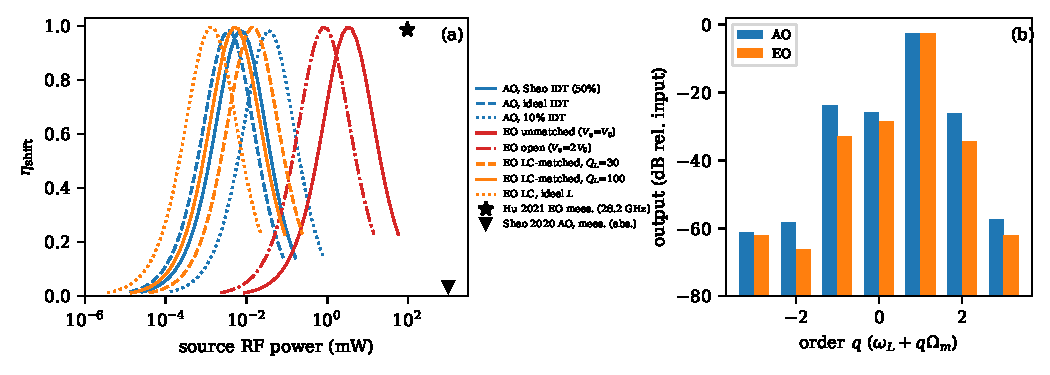
\includegraphics[width=\textwidth]{figures/figB1_eff_power_spectrum.pdf}
\caption{Simulated operating point ($\gamma/2\pi=0.6$~GHz, $\kappa_i/2\pi=80.75$~MHz). (a)~$\etash$ versus source RF power for the acoustic drive (blue: Shao IDT with $\approx$50\% coupling, ideal IDT, 10\% IDT) and for the EO drive with identical optics (red: unmatched, $V_c=V_0$, and open capacitor, $V_c=2V_0$; orange: LC matched with inductor $Q_L=30$, $Q_L=100$, and an ideal inductor). Symbols mark measured devices: the EO shifter of Ref.~\cite{Hu2021} (star; 98.7\% at 96~mW and 28.2~GHz) and the acousto-optic shifter of Ref.~\cite{Shao2020} (triangle; 3.5\% on-chip efficiency at 1~W, which is an absolute rather than a shift-ratio efficiency). (b)~Output power in each order $q$ relative to the input at the respective optima of the AO and EO drives.}
\label{fig:power}
\end{figure*}

\emph{Operating point.}---At $\gamma/2\pi=0.6$~GHz the acoustic drive reaches its maximum $\etash=98.3\%$ at $\delta\omega/2\pi=0.55$~GHz, i.e.\ a source peak voltage of 26~mV and $\Pg=6.7~\mu$W with the Shao IDT (Table~\ref{tab:main}, Fig.~\ref{fig:power}). The absolute efficiency is 55\% and the IL is 2.5~dB; both are set by the intrinsic loss rather than by the drive. The shifted line is the $q=+1$ order. Relative to it, the carrier is at $-23.2$~dB and the largest spurious order is $q=-1$ at $-21.2$~dB ($q=+2$ at $-23.6$~dB). These spurs come from the common-mode phase modulation of single-ring driving. The push-pull EO drive cancels this term and reaches $\etash=99.6\%$, with the carrier at $-26.0$~dB and the $q=-1$ order at $-30.6$~dB [Fig.~\ref{fig:power}(b)], and the same 2.5~dB IL.

\begin{table}[b]
\caption{Simulated operating points at $\gamma/2\pi=0.6$~GHz, $\kappa_i/2\pi=80.75$~MHz (\texttt{data/results\_B.json}) and the measured EO shifter of Ref.~\cite{Hu2021}.}
\label{tab:main}
\begin{ruledtabular}
\small
\begin{tabular}{lccc}
 & AO & EO$^{a}$ & Hu~\cite{Hu2021}\\
 & (sim.) & (sim.) & (meas.)\\
\hline
$\Omega_m/2\pi$ (GHz) & 3.33 & 3.33 & 28.2\\
$\gamma/2\pi$ (GHz) & 0.60 & 0.60 & 5.31\\
$\kappa_i/2\pi$ (MHz) & 80.75 & 80.75 & 170\\
$\etash$ & 98.3\% & 99.6\% & 98.7\%\\
$\etaabs$ & 55\% & 56\% & ---\\
IL (dB) & 2.5 & 2.5 & 0.45\\
Carrier (dB)$^{g}$ & $-23.2$ & $-26.0$ & ---\\
Largest spur (dB)$^{g}$ & $-21.2$ & $-30.6$ & ---\\
$\Pg$, as-built feed & 6.7~$\mu$W$^{b}$ & 3.1~mW$^{c}$ & 96~mW\\
$\Pg$, matched feed & 3.4~$\mu$W$^{d}$ & 1.2--13~$\mu$W$^{e}$ & ---\\
RF bandwidth & $\sim$1~MHz & $\approx$122~MHz$^{f}$ & $>$3~GHz\\
\end{tabular}
\end{ruledtabular}
\raggedright\footnotesize $^{a}$Push-pull, same optics. $^{b}$Shao IDT ($\approx$50\% coupling). $^{c}$$V_c=V_0$. $^{d}$Ideal IDT. $^{e}$LC match, ideal inductor to $Q_L=30$. $^{f}$LC match with $Q_L=30$; the unmatched electrode is broadband. $^{g}$Relative to the shifted line.
\end{table}

\emph{Comparison with EO driving.}---Table~\ref{tab:power} lists the source power at the respective optima for each feed. Without any matching on the EO side ($V_c=V_0$) the EO drive needs 3.1~mW, $\approx$460 times the 6.7~$\mu$W of the acoustic drive, and the measured device of Ref.~\cite{Hu2021} used 96~mW. These factors, however, compare a resonantly enhanced acoustic drive with a non-resonant electrode, and they do not survive a like-for-like comparison. With an LC match the EO power falls to 13~$\mu$W ($Q_L=30$), 4.8~$\mu$W ($Q_L=100$), or 1.2~$\mu$W (ideal inductor). Against the ideally matched IDT (3.4~$\mu$W), the two drives therefore differ only by a factor of 0.36--3.9, and \emph{the EO drive is the more power-efficient one when the inductor loss is low}. Against the as-measured Shao IDT (6.7~$\mu$W) the range is 0.18--1.9. We therefore make no claim of a power advantage over EO driving. The remaining differences are qualitative: the acoustic resonator provides voltage gain without an external matching network, but at the cost of a $\sim$100-fold narrower RF bandwidth (Sec.~\ref{sec:tol}) and a fixed shift frequency.

\begin{table}[t]
\caption{Source RF power at the optimum $\etash$ (simulation; \texttt{data/results\_B.json}, \texttt{data/eff\_vs\_power.csv}).}
\label{tab:power}
\begin{ruledtabular}
\begin{tabular}{lc}
Drive and feed & $\Pg$\\
\hline
AO, Shao IDT ($\approx$50\%) & 6.7~$\mu$W\\
AO, ideal IDT (100\%) & 3.4~$\mu$W\\
AO, 10\% IDT & 34~$\mu$W\\
EO, unmatched ($V_c=V_0$) & 3.1~mW\\
EO, open capacitor ($V_c=2V_0$) & 0.77~mW\\
EO, LC match, $Q_L=30$ & 13~$\mu$W\\
EO, LC match, $Q_L=100$ & 4.8~$\mu$W\\
EO, LC match, ideal inductor & 1.2~$\mu$W\\
\hline
Hu \emph{et al.}~\cite{Hu2021} (meas., 28.2~GHz) & 96~mW\\
\end{tabular}
\end{ruledtabular}
\end{table}

\emph{Comparison with acousto-optic shifters.}---Within the acousto-optic class the design is far ahead of published devices. The best measured TFLN acousto-optic shifter reaches 3.5\% on-chip efficiency at 30~dBm (1~W)~\cite{Shao2020}; the present design reaches $\etaabs=55\%$ ($\etash=98.3\%$) at 6.7~$\mu$W. The comparison is not like for like: Ref.~\cite{Shao2020} is a broadband, non-resonant traveling-wave deflector with a 70-MHz microwave bandwidth, whereas our design trades bandwidth for double (optical and acoustic) resonance. Zhu \emph{et al.}~\cite{Zhu2025ao} operate an acoustic photonic molecule at milliwatt acoustic power in a backward, reflective geometry and do not report a forward shift efficiency or insertion loss. Table~\ref{tab:sota} summarizes these benchmarks.

\begin{table*}[t]
\caption{Benchmarks. ``Meas.'' denotes measured devices, ``sim.'' this work; LNOS, LN-on-sapphire; BW, RF bandwidth. All except Ref.~\cite{Zhu2025ao} are on TFLN. The efficiencies are not all defined identically (see notes).}
\label{tab:sota}
\begin{ruledtabular}
\footnotesize
\begin{tabular}{llllll}
Work & Mechanism & Shift & Efficiency & Drive & Note\\
\hline
Shao \emph{et al.}~\cite{Shao2020} (meas.) & AO traveling wave & $\sim$3~GHz & 3.5\% on-chip$^{a}$ & 1~W (30~dBm) & 70~MHz BW\\
Zhu \emph{et al.}~\cite{Zhu2025ao} (meas.) & AO backward Brillouin (LNOS) & 8.54~GHz & reflectivity $\le$24\% & mW (acoustic) & no forward $\etash$\\
Hu \emph{et al.}~\cite{Hu2021} (meas.) & EO photonic molecule & 28.2~GHz & $\etash=98.7\%$ & 96~mW & IL 0.45~dB, $>$3~GHz BW\\
Qiu \emph{et al.}~\cite{Qiu2025} (meas.) & EO serrodyne & --- & $>$98.8\% & $V_\pi\approx2.3$~V & broadband$^{b}$\\
This work (sim.) & AO photonic molecule & 3.33~GHz & $\etash=98.3\%$, $\etaabs=55\%$ & 6.7~$\mu$W & IL 2.5~dB, $\sim$1~MHz BW\\
EO ref.\ (sim.) & EO molecule, LC matched & 3.33~GHz & $\etash=99.6\%$ & 1.2--13~$\mu$W & 122~MHz BW ($Q_L=30$)\\
\end{tabular}
\end{ruledtabular}
\raggedright\footnotesize $^{a}$Deflected power divided by transmitted power with the microwave off~\cite{Shao2020}. $^{b}$Values taken from the published abstract of Ref.~\cite{Qiu2025}.
\end{table*}

% ================================================================ Tolerance
\section{Tolerances}\label{sec:tol}
\begin{figure*}[t]
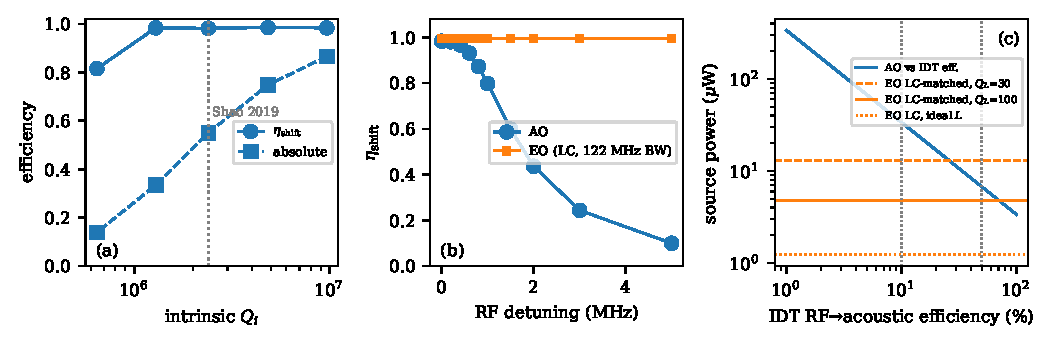
\includegraphics[width=\textwidth]{figures/figB2_tolerance_IDT.pdf}
\caption{Tolerances of the acoustic design (simulation). (a)~$\etash$ (circles) and $\etaabs$ (squares) versus intrinsic $Q_i$, with $\delta\omega$ re-optimized at each point; the dotted line marks the $Q_i$ implied by Ref.~\cite{Shao2019}. (b)~$\etash$ versus RF detuning of the drive from the doublet splitting. For AO the drive amplitude follows the acoustic Lorentzian ($Q_m=2000$, FWHM 1.67~MHz); the EO curve assumes a flat drive within the 122-MHz bandwidth of the $Q_L=30$ LC match. (c)~Source power of the acoustic drive versus IDT RF-to-acoustic efficiency, compared with the LC-matched EO drive (horizontal lines). Dotted vertical lines mark 10\% and 50\%.}
\label{fig:tol}
\end{figure*}

\emph{Optical quality factor.}---Because the coupling $\gamma$ is fixed while $\kappa_i$ varies, the shift ratio is robust but the loss is not [Fig.~\ref{fig:tol}(a)]. For $Q_i\gtrsim1.3\times10^6$ we find $\etash\approx98\%$; at $Q_i=6.4\times10^5$ it drops to 82\%. The absolute efficiency rises from 33\% at $Q_i=1.3\times10^6$ through 55\% at $2.4\times10^6$ to 87\% at $9.7\times10^6$ (IL 0.56~dB). The required source power stays between 6.1 and 8.5~$\mu$W over this range.

\emph{RF detuning.}---The acoustic resonance filters the drive. With $Q_m=2000$ (FWHM 1.67~MHz) we find $\etash\ge96.7\%$ within $\pm0.4$~MHz of the doublet splitting, 80\% at 1~MHz, 44\% at 2~MHz, and 10\% at 5~MHz [Fig.~\ref{fig:tol}(b)]. The usable RF bandwidth is thus $\sim$1~MHz. Under the flat-drive assumption, the LC-matched EO drive keeps $\etash=99.6\%$ over the full $\pm5$~MHz range.

\emph{IDT efficiency.}---The acoustic source power scales as $1/\eta_{\rm IDT}$ [Fig.~\ref{fig:tol}(c)]: 3.4~$\mu$W at 100\%, 6.7~$\mu$W at the Shao IDT's $\approx$50\%, and 34~$\mu$W at 10\%, a value reported for other LN acousto-optic microrings~\cite{Xu2025b}. The acoustic drive needs more power than the $Q_L=30$ LC-matched EO drive (13~$\mu$W) once $\eta_{\rm IDT}\lesssim25\%$, more than the $Q_L=100$ match (4.8~$\mu$W) below $\approx$70\%, and more than the ideal-inductor match (1.2~$\mu$W) for any physical $\eta_{\rm IDT}\le100\%$.

% ================================================================ Quantum
\section{Single-photon performance}\label{sec:quantum}
\emph{HOM visibility.}---A frequency shifter for quantum networks must preserve the spectral-temporal mode of the photon. We model an input photon with a Gaussian spectral amplitude $\psi(\Delta)\propto\exp(-\Delta^2/4\sigma^2)$, where $\sigma$ is the rms width of $|\psi|^2$, and compute the complex transfer function $H(\Delta)$ of the shifted ($q=+1$) channel from the full time-domain solution of Eq.~\eqref{eq:eom} at the AO operating point, evaluated on 41 points over $\pm4\sigma$ (\texttt{data/H\_shift.csv}). The shifted photon, filtered to its target frequency bin, interferes with a reference photon of the same spectrum at the target frequency. Because a fixed delay of the reference can always be added, we maximize over the delay $\tau$:
\begin{equation}
V=\max_\tau\frac{\big|\int\psi^*(\Delta)H(\Delta)\psi(\Delta)e^{-2\pi i\Delta\tau}d\Delta\big|^2}{\int|\psi|^2d\Delta\int|H\psi|^2d\Delta}.
\label{eq:hom}
\end{equation}
The normalization by $\int|H\psi|^2$ assumes that the loss is balanced, e.g.\ by attenuating the reference arm, so $V$ measures mode distinguishability only. The optimum delay is 1.0--1.1~ns, i.e.\ the group delay of the device.

\begin{figure}[t]
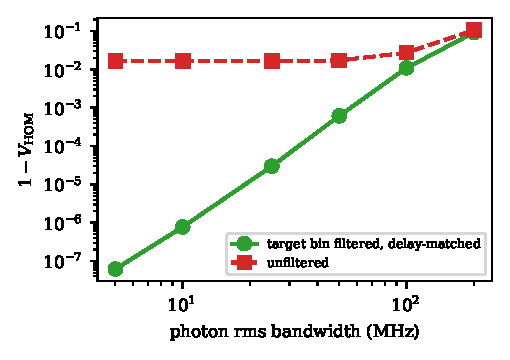
\includegraphics[width=\columnwidth]{figures/figB3_HOM.pdf}
\caption{HOM infidelity $1-V$ versus photon rms bandwidth $\sigma$ (simulation; \texttt{data/HOM.csv}). Circles: shifted photon filtered to the target bin, reference photon delay-matched [Eq.~\eqref{eq:hom}]. Squares: unfiltered, where the residual unshifted and spurious orders limit $V$ to $\approx\etash$.}
\label{fig:hom}
\end{figure}

The results are shown in Fig.~\ref{fig:hom}. With filtering, $1-V=8\times10^{-7}$ at $\sigma=10$~MHz, $3\times10^{-5}$ at 25~MHz, $6\times10^{-4}$ at 50~MHz, $1.1\times10^{-2}$ at 100~MHz, and $9\times10^{-2}$ at 200~MHz. The residual distinguishability comes from the curvature of $H(\Delta)$ beyond linear phase across the photon spectrum, which grows rapidly as $\sigma$ becomes a sizable fraction of the optical linewidths ($\gamma/2\pi=0.6$~GHz). Without filtering, the residual carrier and spurious orders limit the visibility to $V\approx\etash$: $V=0.9835$ at $\sigma=10$~MHz and 0.9829 at 50~MHz, i.e.\ $1-V\approx1.7\times10^{-2}$, more than four orders of magnitude worse than the filtered value at 10~MHz ($V=0.9999992$). A spectral filter on the target bin is therefore required for high-visibility operation. The device is therefore suited to narrowband photons with $\sigma\lesssim50$~MHz, such as cavity-enhanced parametric sources or atom- and quantum-dot-like emitters, together with a spectral filter on the target bin. Broadband photons require a wider optical linewidth, i.e.\ a larger $\gamma$ and correspondingly larger drive.

\emph{Thermal phonons.}---The shift is a pump-free, number-conserving, beam-splitter-type process: the acoustic field scatters a photon from the S to the AS supermode, and no photon is created without an input photon. Thermal occupation $n_{\rm th}$ of the acoustic mode therefore adds only an incoherent fluctuation of the coupling, of relative size $n_{\rm th}/N_{\rm coh}$, where $N_{\rm coh}=(4\gamma_e/\gamma^2)\,\Pg/\hbar\Omega_m$ is the coherently driven phonon number. With $\gamma=\Omega_m/Q_m$, $Q_m=2000$, and $\gamma_e/\gamma=0.15$~\cite{Shao2019}, we find $N_{\rm coh}\approx1.75\times10^{11}$ at the operating point. At 3.33~GHz, $n_{\rm th}=1877$ at 300~K, 24.5 at 4~K, and $1.1\times10^{-7}$ at 10~mK, so $n_{\rm th}/N_{\rm coh}=1.1\times10^{-8}$, $1.4\times10^{-10}$, and $7\times10^{-19}$, respectively. Thermal-phonon noise is therefore negligible even at room temperature, unlike microwave-to-optical transduction, in which thermal phonons are converted into noise photons. We did not model spontaneous scattering of photons into other optical modes by thermal phonons; with the single-phonon coupling $g_0/2\pi\approx1.1$~kHz of this platform~\cite{Shao2019} we expect it to be much smaller than the effects above, but this remains to be quantified.

% ================================================================ Limitations
\section{Limitations}\label{sec:lim}
The results above are design predictions subject to the following limitations.

(i)~\emph{No power advantage over matched EO.} With impedance matching on both sides the acoustic and EO source powers differ only by a factor of 0.36--3.9, and the LC-matched EO drive is more power-efficient with a low-loss inductor (Sec.~\ref{sec:results}). The advantage claimed here is restricted to the class of acousto-optic frequency shifters.

(ii)~\emph{Narrow RF bandwidth and fixed shift frequency.} The usable RF bandwidth is $\sim$1~MHz, set by the acoustic $Q_m=2000$, versus $\approx$122~MHz for a $Q_L=30$ LC-matched EO electrode and $>$3~GHz for the unmatched device of Ref.~\cite{Hu2021}. The shift is fixed at the 3.33-GHz acoustic resonance, whereas EO photonic molecules have been operated at 12.5--28.2~GHz~\cite{Hu2021}. The RF source must be frequency-stabilized, and the doublet splitting must be thermally tuned to match $\Omega_m$ to well within the optical linewidth.

(iii)~\emph{Insertion loss.} The IL is 2.5~dB ($\etaabs=55\%$), limited by the measured $Q_i\approx2.4\times10^6$ of the suspended platform~\cite{Shao2019}, compared with 0.45~dB for the measured EO device~\cite{Hu2021}.

(iv)~\emph{IDT efficiency.} The acoustic drive loses to a $Q_L=30$ LC-matched EO drive if the IDT efficiency is below $\approx$25\%; IDT efficiencies of $\approx$10\% have been reported in related LN microring devices~\cite{Xu2025b}.

(v)~\emph{Drive extrapolation.} We obtain $\delta\omega$ by extrapolating the measured MZI $V_\pi L$ of Ref.~\cite{Shao2019} linearly to a ring that the acoustic field covers only partially (15\%). We assume the same IDT efficiency, mode overlap, and uniform acoustic phase along the covered section as in the MZI. This extrapolation must be verified experimentally; $n_g=2.3$ is assumed.

(vi)~\emph{Not modeled.} We did not model optical loss from the IDT metal or the suspended region, ohmic and acoustic heating of the IDT and resonator, the resulting thermo-optic drift of the ring resonances (Ref.~\cite{Shao2019} observed a heating-induced red shift with increasing microwave power), or the mechanical stability of the suspended structure.

(vii)~\emph{Model provenance.} Our implementation of Eq.~\eqref{eq:eom} is reconstructed from the published equations of Ref.~\cite{Hu2021}, not from the authors' code, and the design combines parameters of two different devices (optics and electrodes from Ref.~\cite{Hu2021}, acoustics and loss from Ref.~\cite{Shao2019}). Any extension that routes the acoustic drive through on-chip phononic circuits (for example, to feed several shifters) would at present rely on acoustic-circuit parameters borrowed from GaN-on-sapphire~\cite{Xu2025} and on our reconstruction of that model from its equations; none of the numbers reported here depend on it.

% ================================================================ Conclusion
\section{Conclusion}
In simulation, a suspended IDT acoustic resonator driving one ring of a TFLN photonic molecule shifts 98.3\% of the output light by 3.33~GHz at $\approx$7~$\mu$W of source power, with 55\% absolute efficiency and 2.5~dB insertion loss. This is orders of magnitude beyond the best published acousto-optic shifter (3.5\% at 1~W~\cite{Shao2020}) and, unlike the backward-Brillouin photonic molecule of Ref.~\cite{Zhu2025ao}, operates as a forward, single-bus shifter. It is not more power-efficient than an impedance-matched EO drive of the same optics (factor 0.36--3.9, EO better with low-loss inductors), and it has a $\sim$1-MHz RF bandwidth and a fixed shift frequency. With a delay-matched reference and filtering of the target bin, the HOM infidelity is $8\times10^{-7}$ for 10-MHz and $6\times10^{-4}$ for 50-MHz photons (unfiltered, $V=0.9835$ at 10~MHz), and thermal phonon noise is negligible at room temperature. The decisive experiments are a measurement of the acousto-optic coupling of a partially covered high-$Q$ ring, together with the IDT efficiency and the loss and heating added by the IDT.

\emph{Data availability.}---Simulation scripts (\texttt{core.py}, \texttt{make\_all.py}, \texttt{hom\_post.py}) and data files are available from the author.

\bibliography{refs}

\end{document}
